\section{Markov Model}\label{sec:models}

Navigating through a web site can be seen as a sequence of states where a pair of states are connected. One can simulate a tree representation of the web site where the root of the tree will be the domain (main page) and the leafs the deepest paths a user can reach.
\\[2ex]
This was the inspiration to represent the training data: we convert training data into a graph representation.~\cite{article:markovmodel} Each fragment of the URL corresponds to one node. All the possible previous and next fragments of the URL are connected to the current fragment by connecting the nodes with edges. Each node and edge contains the amount of times it was traversed. The occurrences are then used to compute the probabilities. Our model is a Markov chain model.~\footnote{\url{https://en.wikipedia.org/wiki/Markov_chain}} Figure~\ref{fig:markov_chain} illustrates the concept.
\\[2ex]
An important consideration here was creating a Markov chain model for each domain separately. The reason we do this is because we are only interested in the end path within a specific domain and not in the previous or next domain. The chance with which we get to a certain domain becomes irrelevant because we only need the probabilities when the domain is already given (when the user loads a page).

\begin{figure}[!htp]
	\centering
	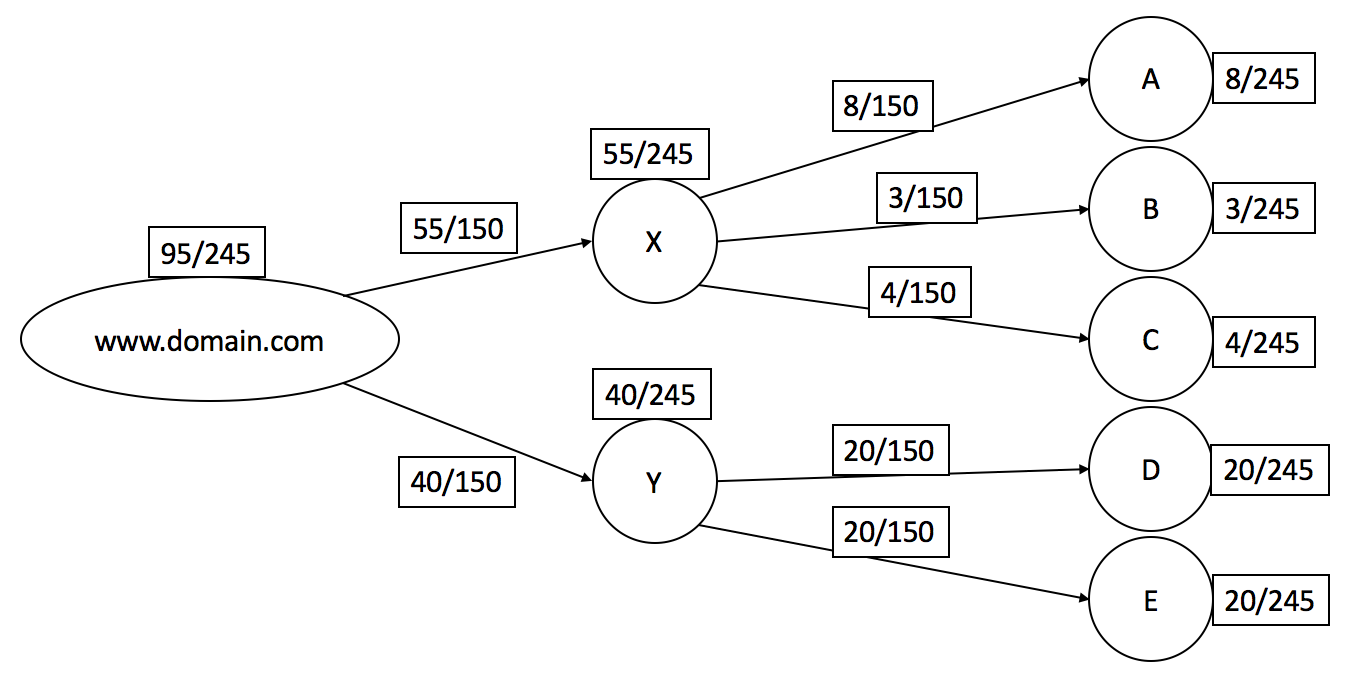
\includegraphics[width=\textwidth]{markov_chain}
	\caption{Markov chain model representation}\label{fig:markov_chain}
\end{figure}

The goal of our model is not only to predict the most likely deepest path but also to make the prediction as fast as possible. The hill climbing search in Markov hill climbing model was implemented to achieve this.~\cite{lopez2008heuristic} The hill climbing search is set up with a memory of one node and works as follows:

\begin{enumerate}
	\item Receive the graph model and the current state/path were we need to predict. This path is not limited to the first page of the website.
	\item Store the current path.
	\item Take the next states connected to the current state.
	\item Compute the difference between of the probabilities of the states. If the difference is greater than the confidence interval, then the state is discarded.
	\item If there is more than one next possible state, take the one with the highest transition probability and update the current path.
	\item Repeat steps 3, 4 and 5 until there are no next states of the current path or we discard all the next states in step 4.
\end{enumerate}

Step 4 is an important aspect of our model because we want the deepest useful path to be predicted. Take again for example figure~\ref{fig:markov_chain}. Let's say we wish to predict the next page for \textit{www.domain.com/X}. If the domain interval is low enough (i.e. 0.2), then A will be predicted because it has the highest chance: $8/(8+3+4) \approx 50\%$. But if the confidence interval is set high (i.e. 0.6), then none of the endpaths are eligible anymore and no deeper path will be found. A thorough explanation on this matter can be consulted in section~\ref{sec:truth}.

TODO

www.domain.com represents the very first page of the web site, if the confident interval is setup as 1, the result of the search will be the path www.domain.com/X/A, however, according with the state probabilities, most of the time user stays in path www.domain.com/X, which probably it is more useful than www.domain.com/X/A. Now I we use our search method with a confident interval of 15\% the result of our search will be www.domain.com/X since the delta between state X and the next states connected with it are less that our confident interval.
\\[2ex]
When we ran our model with one of the possible scenarios, we kept track of those correct and incorrect predictions and then we computed the accuracy of our predictions, which is the total correct prediction divided by the total of predictions made. 
\\[2ex]
We also added a simulation of incremental learning in our model, each time we made a prediction we reinforced the graph with the real url that the user wants to visit according with our ground truth. We incremented the probabilities of such url (the correct path) in every iteration.

The transition matrices for each Markov chain are relatively compact since they only represent one domain each. We originally used one single Markov chain for the entire dataset, which computed an enormous sparse transition matrix. A big matrix with very little useful information scattered all over is not very efficient to work with. The individual Markov chains reduce this a lot. The performance is also further improved from the data filtering we did before: there is no point in creating Markov chains for websites we are not interested in. Since the data is compact and the performance does not increase a lot with size, this makes our program very scalable.
\\[2ex]
In order to be called a strong scalable program, the performance must be maintained over time. We only used the timestamps of our datasets to define sessions and to preserve the ordering of the actions. The timestamps are not taken into consideration for the prediction itself. The consequence is that we take a simplistic approach in computing the predictions and require little data to do so. We potentially sacrifice a bit of accuracy in favor of more performance and less storage.
\\[2ex]
It's worth noting that we had originally tried to implement a Hidden Markov Model, using the \textit{hmmlearn} module.~\footnote{\url{https://en.wikipedia.org/wiki/Hidden_Markov_model}}\footnote{\url{https://github.com/hmmlearn/hmmlearn}} But since the states (endpaths) we are looking for are not hidden and we are not interested in computing the probabilities of extra (hidden) attributes, we decided the extra complexity is unnecessary.

\subsection{Model test}\label{subsec:model_test}

The first attempt to make predictions we used was using the Hidden Markov Model of the library hmmlearn, however we realised that such approach was out of the scope, we found that Hidden Markov Model is on the top of the Markov chain model, making prediction where are taking into account not only the probabilities of the edges but also the probabilities of extra attribute of the states, for instances on variable to predict the most likely deepest path could be the mood of the user.
\\[2ex]
As an alternative solution, we considered the idea of~\cite{article:markovmodel}, we thought that simple deep-first method is not the most accurate for this purpose. The goal of our model is not predict the most likely deepest path but also make the prediction as fast as possible, method hill climbing search in markov hill climbing model was implemented to achieve so.
\\[2ex]
Method hill climbing search is based  on the hill climbing search method, hill climbing method is setup with a memory of one node and works as follow:

\begin{enumerate}
  \item Receives the graph model and the current state/path were we need to predict, such path it is not limited to be the very first page of the web site
  \item Stores the current path
  \item Takes the next states connected to the current state
  \item Computes the delta between of the probabilities of the states, if such delta is greater of the confident interval such state is discarded.
  \item If there are more than one next possible state, takes the one with the highest transition probability and updates the current path
  \item Repeats step 3,4 and 5 until there is no next states of the current path or we discard all the next states in step 4.
\end{enumerate}

Step 4 is an important aspect of our model because we want the most deepest useful path to be predicted, for example, we can have the following Markov chain model of a given domain: (figure~\ref{fig:markov_chain})



www.domain.com represents the very first page of the web site, if the confident interval is setup as 1, the result of the search will be the path www.domain.com/X/A, however, according with the state probabilities, most of the time user stays in path www.domain.com/X, which probably it is more useful than www.domain.com/X/A. Now I we use our search method with a confident interval of 15\% the result of our search will be www.domain.com/X since the delta between state X and the next states connected with it are less that our confident interval.
\\[2ex]
When we ran our model with one of the possible scenarios, we kept track of those correct and incorrect predictions and then we computed the accuracy of our predictions, which is the total correct prediction divided by the total of predictions made. 
\\[2ex]
We also added a simulation of incremental learning in our model, each time we made a prediction we reinforced the graph with the real url that the user wants to visit according with our ground truth. We incremented the probabilities of such url (the correct path) in every iteration.

\subsection{Results}\label{subsec:results}
The result for the naive scenarios shows us that this method is not finest one. The more percentage of training data we give to our model, the more accuracy we get. This could interpreted as an overfitting of our data in our model. We can also need to consider that the data is split them randomly, in some user the accuracy of the data is high because of the set of training and testing data was split consistency, while in some user have the bad luck to have the training data and the test data with a very few relationship between them. This just confirmed our assumptions that this naive method is not the best for training and testing our model.
\\[2ex]
In the other hand, the result when we used the k fold cross validation was much consistent, if use the same confident interval with either incremental learning or non incremental learning and we test test our model, we almost obtain the same accuracy for each k fold configuration. After knowing that the k fold give us uniform result, we obtain the best accuracy where the confident interval is set in 20\%. Finally we obtained that the incremental learning increases slightly the accuracy of our model, in fact this is what we expected, since the amount of testing data is relatively small to actually learn from it. The more testing data we have, the more be can improve our model.